\section{Introduction}
\lipsum[2]
\lipsum[3]


\section{Headings: first level}
\label{sec:headings}

\lipsum[7] See Section \ref{sec:headings}.

\subsection{Headings: second level}
\lipsum[5]
\begin{equation}
\xi _{ij}(t)= {\frac {\alpha _{i}(t)a^{w_t}_{ij}\beta _{j}(t+1)b^{v_{t+1}}_{j}(y_{t+1})}{\sum _{i=1}^{N} \sum _{j=1}^{N} \alpha _{i}(t)a^{w_t}_{ij}\beta _{j}(t+1)b^{v_{t+1}}_{j}(y_{t+1})}}
\end{equation}

\begin{figure}[H]
  \centering
  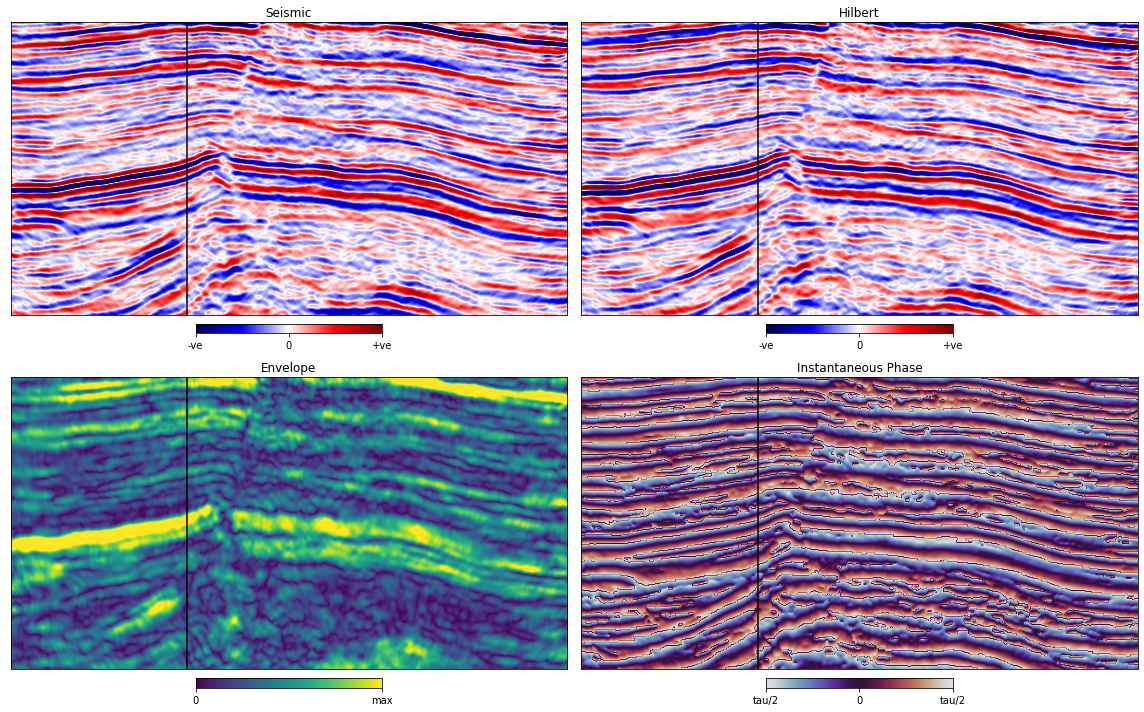
\includegraphics[width=1.0\linewidth]{seismic-figure.png}
  \caption{Sample figure caption.}
  \label{fig:fig1}
\end{figure}

\subsubsection{Headings: third level}
\lipsum[6]

\paragraph{Paragraph}
\lipsum[7]

\section{Examples of citations, figures, tables, references}
\label{sec:others}
\lipsum[8] \cite{kour2014real,kour2014fast} and see \cite{hadash2018estimate}.

The documentation for \verb+natbib+ may be found at
\begin{center}
  \url{http://mirrors.ctan.org/macros/latex/contrib/natbib/natnotes.pdf}
\end{center}
Of note is the command \verb+\citet+, which produces citations
appropriate for use in inline text.  For example,
\begin{verbatim}
   \citet{hasselmo} investigated\dots
\end{verbatim}
produces
\begin{quote}
  Hasselmo, et al.\ (1995) investigated\dots
\end{quote}

\begin{center}
  \url{https://www.ctan.org/pkg/booktabs}
\end{center}

\subsection{Figures}
\lipsum[10]
See Figure \ref{fig:fig1}. Here is how you add footnotes. %\footnote{Sample of the first footnote.}
\lipsum[11]

\subsection{Tables}
\lipsum[12]
See awesome Table \ref{tab:table}.

\begin{table}[H]
 \caption{Sample table title}
  \centering
  \begin{tabular}{lll}
    \toprule
    \multicolumn{2}{c}{Part}                   \\
    \cmidrule(r){1-2}
    Name     & Description     & Size ($\mu$m) \\
    \midrule
    Dendrite & Input terminal  & $\sim$100     \\
    Axon     & Output terminal & $\sim$10      \\
    Soma     & Cell body       & up to $10^6$  \\
    \bottomrule
  \end{tabular}
  \label{tab:table}
\end{table}

\subsection{Lists}
\begin{itemize}
\item Lorem ipsum dolor sit amet
\item consectetur adipiscing elit.
\item Aliquam dignissim blandit est, in dictum tortor gravida eget. In ac rutrum magna.
\end{itemize}

%%%%%%%%%%%% Supplementary Methods %%%%%%%%%%%%
%\footnotesize
%\section*{Methods}
